\documentclass[17pt]{beamer} %Makes presentation
%\documentclass[handout]{beamer} %Makes Handouts
\usetheme{Singapore} %Gray with fade at top
\useoutertheme[subsection=false]{miniframes} %Supppress subsection in header
\useinnertheme{rectangles} %Itemize/Enumerate boxes
\usecolortheme{seagull} %Color theme
\usecolortheme{rose} %Inner color theme

\definecolor{light-gray}{gray}{0.75}
\definecolor{dark-gray}{gray}{0.55}
\setbeamercolor{item}{fg=light-gray}
\setbeamercolor{enumerate item}{fg=dark-gray}

\setbeamertemplate{navigation symbols}{}
%\setbeamertemplate{mini frames}[default]
%\setbeamercovered{dynamics}
\setbeamerfont*{title}{size=\Large,series=\bfseries}
\setbeamerfont{footnote}{size=\tiny}

%\setbeameroption{notes on second screen} %Dual-Screen Notes
%\setbeameroption{show only notes} %Notes Output

\setbeamertemplate{frametitle}{\vspace{.5em}\bfseries\insertframetitle}
\newcommand{\heading}[1]{\noindent \textbf{#1}\\ \vspace{1em}}

\usepackage{bbding,color,multirow,times,ccaption,tabularx,graphicx,verbatim,booktabs}
\usepackage{colortbl} %Table overlays
\usepackage[english]{babel}
%\usepackage[latin1]{inputenc}
%\usepackage[T1]{fontenc}
\usepackage{lmodern}

%\author[]{Thomas J. Leeper}
\institute[]{
  \inst{}%
  Department of Government\\London School of Economics and Political Science
}

\usepackage{tikz}
\usetikzlibrary{shapes,arrows}

\title{Welcome and First Lecture}

\date[]{}

\begin{document}

\frame{\titlepage}

\frame{\tableofcontents}

% An overview of the course and an introduction to political science research. How do we identify research topics to study empirically? What makes for a good political science research questions?

\section{Substantive Material}

\frame{

\frametitle{Claims}

\begin{itemize}\itemsep1em

\item Politics is full of claims

\item The credibility of claims depends on the strength of evidence and argument

\item This class aims to give you tools to:

\begin{itemize}\itemsep1em
\item make credible claims, \textit{and}
\item evaluate claims made by others
\end{itemize}

\end{itemize}

}


\frame{

\frametitle{An Example}

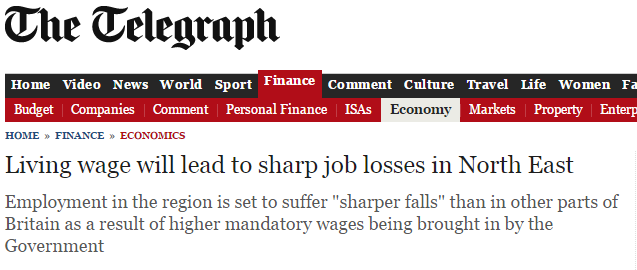
\includegraphics[width=\textwidth]{images/telegraph}

\footnotesize Source: \href{http://www.telegraph.co.uk/finance/economics/11872262/Living-wage-will-lead-to-sharp-job-losses-in-North-East.html}{Peter Spence, \textit{The Telegraph}, Sep. 18, 2015}
}

% is this true or false? ultimately, it doesn't really matter what we think a priori. we have to collect evidence





\frame{

\frametitle{Definitions}

\begin{itemize}\itemsep2em

\item Inference: ``a belief based on evidence \emph{and} rules for processing that evidence''

\item Methodology: ``tools for gathering and analyzing data to try to make valid inferences''

\end{itemize}
}

\begin{frame}[fragile]

\frametitle{Drawing Inferences}

\vspace{-2em}

\begin{center}
\tikzstyle{block} = [rectangle, draw, fill=blue!20!white, text width=5em, text centered, rounded corners, minimum height=4em, node distance=7em]
\begin{tikzpicture}[scale=0.5]
\node<1-> [block] (claims) {Claim(s)};
\node<2-> [block, below of=claims] (beliefs) {Belief(s)};
\node<3-> [block, left of=beliefs] (filter) {Processing Filter};
\node<3-> [block, left of=filter] (evidence) {Evidence};

\draw<3-> [->, very thick] (evidence) -- (filter);
\draw<3-> [->, very thick] (filter) -- (beliefs);
\draw<2-> [->, dashed, very thick] (beliefs) -- (claims);

\draw<4-> [red, very thick] (-12,-8) ellipse (8cm and 4cm);
\draw<4-> (-12,-1) node (topic) {\Large\textcolor{red}{Focus of this class}};
\end{tikzpicture}
\end{center}

\end{frame}



\frame{

\frametitle{Question for you}

\Large How might be draw an inference about the effect of a minimum wage change on the level of unemployment?

}

% minimum wage; unemployment?
% example
% time-series or historical analysis
% comparative analysis across countries or subnational units
% quasi-experimental comparison using a geographical discontinuity
% randomized experiment
% surveys to measure potential employees' willingness to work or employers' willingness to hire (or fire) new employees
% qualitative interviewing

% claims



\frame{

\frametitle{Two Categories of Inference}

\begin{enumerate}\itemsep2em

\item Descriptive Inference

\begin{itemize}
\item What are the facts?
\end{itemize}

\item Causal Inference

\begin{itemize}
\item Why does something occur?
\end{itemize}

\end{enumerate}

}

\frame{

\frametitle{Descriptive Inference}

\begin{itemize}\itemsep0.5em

\item Sometimes seen as the lesser type of inference

\item Still often very interesting

\item Examples

\begin{itemize}
\item Is the climate changing? 
\item Is the United States politically polarized? 
\item Is global terrorism increasing?
\item Is Azerbaijan a democracy?
\end{itemize}

\end{itemize}

}

\frame{

\frametitle{Causal Inference I}

\begin{itemize}\itemsep0.5em

\item Typically what we are interested in

\item Questions about ``why?''

\item Examples

\begin{itemize}
\item \emph{Why} is the climate changing? 
\item \emph{Why} is the United States politically polarized? 
\item \emph{Why} is (or is not) global terrorism increasing?
\item \emph{Why} is (or is not) Azerbaijan a democracy?
\end{itemize}

\end{itemize}

}
\frame{

\frametitle{Causal Inference II}

Typically start with either:

\begin{enumerate}\itemsep1em

\item an outcome (dependent variable)\\
\vspace{1em}
or

\item a cause (independent variable)

\end{enumerate}

}


\begin{frame}
\frametitle{Causal Inference: 2 Types}

\begin{columns}[T] % align columns
\begin{column}{.4\textwidth}
\begin{block}{Reverse}
\small If what, then Y? What causes Y?\\
\vspace{1em}
Associated with a search for causes\\
\vspace{1em}
ex. What causes climate change?\\
\end{block}
\end{column}

\begin{column}{.4\textwidth}
\begin{block}{Forward}
\small If X, then what? What happens if X?\\
\vspace{1em}
Associated with ``Experimentation''\\
\vspace{1em}
ex. What happens if we release greenhouse gases into the air?
\end{block}
\end{column}
\end{columns}

\vspace{1em}
(Gelman 2011)
\end{frame}




% test of distinction between descriptive and causal inference
% discuss with partner
\frame{
\frametitle{Which of these is a causal research question?}

\small

\begin{enumerate}\itemsep0.25em
\item Will Labour win the next UK general election?
\item \textcolor<2->{red}{What had to have happened for Labour to win the last UK general election?}
\item How has Labour's electoral performance changed over the last three decades?
\item What was the result of the last UK general election?
\item \textcolor<3->{red}{What role did the economy have on the last UK general election?}
\end{enumerate}
}




\frame{
\frametitle{Good research questions}

\begin{itemize}\itemsep2.5em
\item Start from political problem or puzzle
\item Builds on an existing research literature
\item Non-obvious\footnote{Note: evolving standard}
\end{itemize}
}
% research topics
% what is ``political''?


% three sets of two example questions (one good; one bad)

\begin{frame}
\frametitle{Which is a better RQ?} % non-obvious

\small

\begin{columns}[T] % align columns
\begin{column}{.4\textwidth}
\begin{block}{}
Why was Germany allocated 96 seats in the European Parliament during the 2014 elections?
\end{block}
\end{column}

\begin{column}{.4\textwidth}
\begin{block}{}
Why was ``degressive proportionality'' chosen as the method of allocating seats in the EP?
\end{block}
\end{column}
\end{columns}

\end{frame}


\begin{frame}
\frametitle{Which is a better RQ?} % builds on literature

\small

\begin{columns}[T] % align columns
\begin{column}{.4\textwidth}
\begin{block}{}
Given what we know from Skocpol about the causes of social revolutions, why haven't such revolutions occurred in several post-Soviet states in Central Asia?
\end{block}
\end{column}

\begin{column}{.4\textwidth}
\begin{block}{}
Given my conversations with taxi drivers during my weekend holiday in Tashkent, why hasn't Uzbekistan become a full-fledged democracy?
\end{block}
\end{column}
\end{columns}

\end{frame}



\begin{frame}
\frametitle{Which is a better RQ?} % starts from a political problem

\small

\begin{columns}[T] % align columns
\begin{column}{.4\textwidth}
\begin{block}{}
How do social media facilitate Britons' decisions about where to take a summer holiday?
\end{block}
\end{column}

\begin{column}{.4\textwidth}
\begin{block}{}
How did social media use shape the development of ``Arab Spring'' protests in Egypt?
\end{block}
\end{column}
\end{columns}

\end{frame}







\frame{
\frametitle{Other ways to generate research questions}

\begin{enumerate}\itemsep1em
\item Puzzle-driven
\item Theory-driven
\item Data-driven
\item Method-driven
\end{enumerate}
}



% purpose of this class is to give you skills to answer research questions/puzzles


\frame{
\frametitle{Scientific method}

\begin{enumerate}
\item Research question(s)
\item Clarify the core concepts % that we're talking about and how we will observe and measure
\item Develop theory
\item Derive specific, testable hypotheses
\item Plan data collection % (different kinds of data for different questions of research questions)
\item Gather data/evidence
\item Analyze data
\item Draw inferences
\end{enumerate}

}



\frame{\huge\vskip20pt\textbf{Questions?}}





\section{Introductions}
\frame{\tableofcontents[currentsection]}

\frame{
\frametitle{Who am I?}

\small

\begin{itemize}\itemsep0.5em

\item Assistant Professor in Political Behaviour

\item Worked in Denmark for past 2.5 years

\item Originally from Minnesota (USA)

\item Interested in public opinion and political psychology

\item Office hours:\\
Tuesday 9--11 CON 3.21\\
Sign-up on LSE for You\\
Otherwise, email: \href{mailto:t.leeper@lse.ac.uk}{t.leeper@lse.ac.uk}

\end{itemize}

}

\frame{
\frametitle{Who is your GTA?}

\begin{itemize}\itemsep1em

\item Bernardo Rangoni

\item 

\end{itemize}

}


\frame{

\frametitle{Who are you?}

\begin{itemize}\itemsep1em

\item Introduce yourself to a neighbour

\item Where are you from?

\item What interests you about government or politics?

\item What do you hope to learn from the course?

\end{itemize}

}



\section{Administrative Stuff}
\frame{\tableofcontents[currentsection]}

\frame{

\frametitle{Course Resources}

\small

\begin{itemize}\itemsep2em
\item Moodle

\item Reading list:
\url{http://readinglists.lse.ac.uk/lists/B821602E-0B75-9923-D8C5-457373E1789E.html}

	\begin{itemize}
	\item Gerring
	\item Kellstedt and Whitten
	\end{itemize}

\end{itemize}

}




\frame{

\frametitle{Schedule: Michaelmas Term}

\footnotesize

1 Introduction (Sep. 28) \\
2 Causality: Explanation versus Prediction (Oct. 6) \\
3 Concepts: ``I'll know it when I see it'' (Oct. 13) \\
4 Measurement: Concepts in Practice (Oct. 20) \\
5 Building and Testing Political Science Theories (Oct. 27) \\
6 Deriving Hypotheses from Theory (Nov. 3) \\
7 Case Studies (Nov. 10) \\
8 Case Comparisons (Nov. 17) \\
9 Causal Mechanisms and Process-Tracing (Nov. 24) \\
10 Texts into Interpretations and Analysis (Dec. 1) \\

}

\frame{

\frametitle{Schedule: Lent Term}

\footnotesize

11 Interviewing, Structured and Unstructured (Jan. 12) \\
12 Participant Observation (Jan. 19) \\
13 Tabulation and Visualization (Jan. 26) \\
14 Sampling and Representativeness (Feb. 2) \\
15 Statistical Inference (Feb. 9) \\
16 Regression Analysis (Feb. 23) \\
17 Matching and Regression
(Mar. 1) \\
18 Experimental Design and Quasi-Experiments
(Mar. 8) \\
19 Ethics and Research Integrity (Mar. 15) \\
20 Conclusion and Synthesis (Mar. 22) \\

}


\frame{

\frametitle{Learning Outcomes}

\small

\begin{enumerate}\itemsep0.75em
\item Identify interesting political science research questions and formulate theories and
hypotheses that answer them
\item Describe and operationalize concepts from political science theories
\item Evaluate the strengths and weaknesses of different approaches to empirical research
\item Apply political science theories to the design of original research
\end{enumerate}

}

\frame{

\frametitle{Summative Assessment}

\begin{enumerate}\itemsep2em
\item Breadth: 2-hour written exam (Summer Term)

\item Depth: 3000-word research design proposal
\end{enumerate}

}

\frame{

\frametitle{Research Design Proposal}

\begin{itemize}\itemsep1em

\item Research question
\item Theoretical contribution
\item Testable hypotheses
\item Description of the proposed data collection and analysis

\vspace{0.5em}

\item Due Date: 
\end{itemize}

}



\frame{

\frametitle{Problem Sets}

\small

\begin{tabular}{ll}
Assignment & Due Date \\ \hline
Concepts and measurement & Tuesday Oct. 27 \\
Theory and hypothesis generation & Tuesday Nov. 10 \\
Case selection & Tuesday Nov. 24 \\
Text analysis & Tuesday Dec. 15 \\
Interviewing & Tuesday Jan. 26 \\
Basic Statistics & Tuesday Feb. 23 \\
Regression analysis & Tuesday Mar. 8 \\
Experimentation & Tuesday Mar. 22 \\
\end{tabular}

}


\frame{\huge\vskip20pt\textbf{Questions?}}


\appendix
\frame{}

\end{document}
